\documentclass[11pt]{article}
\usepackage[utf8]{inputenc}
\usepackage[T1]{fontenc}
\usepackage{amsmath}
\usepackage{multicol}
\usepackage{geometry}
\usepackage{tikz}
\usetikzlibrary{shapes.geometric, arrows.meta}
\usepackage{enumitem}
\usepackage{xcolor}
\usepackage{titlesec}
\usepackage{parskip}       % Espaçamento entre parágrafos
\setlength{\parskip}{0.5em} % Ajuste o valor conforme necessário
\renewcommand{\baselinestretch}{1.0} % Espaçamento entre linhas

% Configurações de layout
\geometry{a4paper, left=1cm, right=1cm, top=0.5cm, bottom=1.2cm}
\setlength{\columnseprule}{0.4pt}
\setlength{\baselineskip}{1.0\baselineskip}

% Cores para títulos
\titleformat{\section}{\normalfont\Large\bfseries\color{blue}}{\thesection}{1em}{}
\titleformat{\subsection}{\normalfont\large\bfseries\color{red}}{\thesubsection}{1em}{}
\titleformat{\subsubsection}{\normalfont\normalsize\bfseries\color{black}}{\thesubsubsection}{1em}{}

\title{\textcolor{blue}{Função Exponencial: Crescimento e Decaimento}}
\author{Professor: Jefferson}
\date{}

\begin{document}

\maketitle
\vspace{-1cm}

\begin{center}
\large{Nome: \underline{\hspace{8cm}} \quad Turma: \underline{\hspace{3cm}}}
\end{center}

\begin{multicols}{2}

\section*{1. Conceito}
Uma função exponencial é expressa por:
\[
f(x) = a \cdot b^x \quad \text{ou} \quad y = a \cdot b^x
\]
onde:
\begin{itemize}
    \item $a$ é o valor inicial ($a \neq 0$)
    \item $b$ é a base ($b > 0$, $b \neq 1$)
    \item $x$ é o expoente (variável independente)
\end{itemize}

\subsection*{Exemplos Característicos}
\begin{itemize}
    \item Crescimento: $f(x) = 2^x$ \quad ($a=1$, $b=2$)
    \item Decaimento: $g(x) = 3 \cdot \left(\frac{1}{2}\right)^x$ \quad ($a=3$, $b=0.5$)
    \item Com deslocamento: $h(x) = 2^{x} - 1$
\end{itemize}

\section*{2. Gráfico: Curva Exponencial}
Características principais:
\begin{itemize}
    \item \textbf{Forma}: Curva suave que cresce/decai rapidamente
    \item \textbf{Assíntota horizontal}: $y = k$ (geralmente $y=0$)
    \item \textbf{Intercepto y}: $(0, a)$
\end{itemize}

\begin{center}
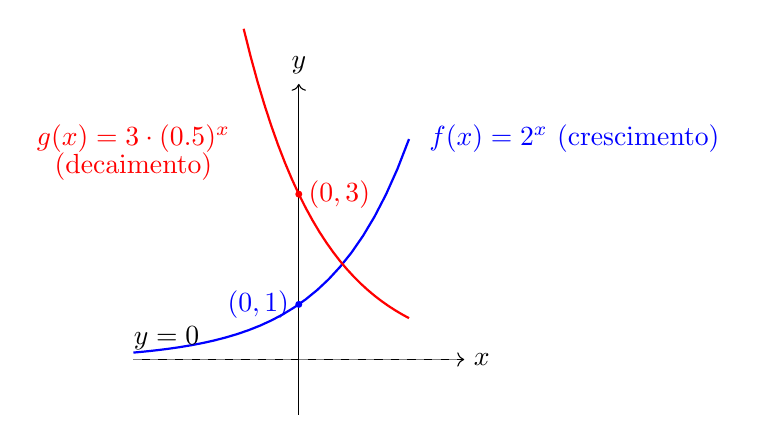
\begin{tikzpicture}[scale=0.7]
    % Eixos
    \draw[->] (-3,0) -- (3,0) node[right]{$x$};
    \draw[->] (0,-1) -- (0,5) node[above]{$y$};
    % Funções
    \draw[blue, thick, domain=-3:2] plot (\x, {2^\x});
    \node[blue] at (5.0,4) {$f(x)=2^x$ (crescimento)};
    \draw[red, thick, domain=-1:2] plot (\x, {3*(0.5^\x)});
    \node[red] at (-3,4) {$g(x)=3\cdot(0.5)^x$};
    \node[red] at (-3,3.5) {(decaimento)};
    % Assíntotas
    \draw[dashed, gray] (-3,0) -- (3,0) node[black, pos=0.1, above]{$y=0$};
    % Pontos
    \filldraw[blue] (0,1) circle (1.5pt) node[left]{$(0,1)$};
    \filldraw[red] (0,3) circle (1.5pt) node[right]{$(0,3)$};
\end{tikzpicture}
\end{center}

\section*{3. Comportamento da Função}
\begin{itemize}
    \item \textbf{Base $b > 1$}:
    \begin{itemize}
        \item Função crescente
        \item Domínio: $\mathbb{R}$
        \item Imagem: $(0, +\infty)$
    \end{itemize}
    
    \item \textbf{Base $0 < b < 1$}:
    \begin{itemize}
        \item Função decrescente
        \item Domínio: $\mathbb{R}$
        \item Imagem: $(0, +\infty)$
    \end{itemize}
\end{itemize}

\begin{center}
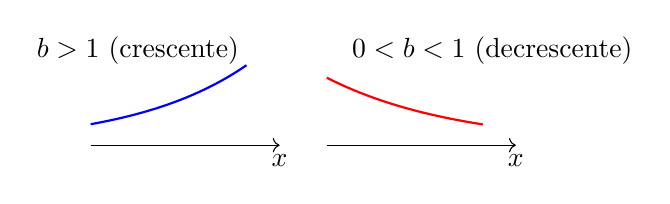
\begin{tikzpicture}[scale=0.6]
    % Crescimento (b > 1)
    \draw[->] (-2,0) -- (2,0) node[below]{$x$};
    \draw[blue, thick, domain=-2:1.3] plot (\x, {1.5^\x});
    \node at (-1,2) {$b>1$ (crescente)};
    % Decaimento (0 < b < 1)
    \draw[->] (3,0) -- (7,0) node[below]{$x$};
    \draw[red, thick, domain=-1:2.3] plot (\x+4, {0.7^\x});
    \node at (6.5,2) {$0<b<1$ (decrescente)};
\end{tikzpicture}
\end{center}

\section*{4. Propriedades Fundamentais}
Para $a > 0$ e $b > 0$ ($b \neq 1$):
\begin{enumerate}
    \item $b^{x+y} = b^x \cdot b^y$
    \item $b^{x-y} = \frac{b^x}{b^y}$
    \item $(b^x)^y = b^{x \cdot y}$
    \item $a^x = b^{x \cdot \log_b a}$
\end{enumerate}

\section*{5. Zero da Função}
A função exponencial \textbf{nunca tem zeros} quando:
\[
f(x) = a \cdot b^x \quad (a \neq 0, b > 0)
\]
Pois $b^x > 0$ para todo $x \in \mathbb{R}$.

\subsection*{Exceção com Transformações}
Se houver deslocamento vertical:
\[
f(x) = a \cdot b^x + k
\]
O zero ocorre quando:
\[
a \cdot b^x + k = 0 \Rightarrow b^x = -\frac{k}{a}
\]
(Só existe solução se $-\frac{k}{a} > 0$)

\section*{6. Aplicações Práticas}
\subsection*{Crescimento Populacional}
Modelo de crescimento:
\[
P(t) = P_0 \cdot e^{rt}
\]
onde:
\begin{itemize}
    \item $P_0$: população inicial
    \item $r$: taxa de crescimento
    \item $t$: tempo
\end{itemize}

\subsection*{Decaimento Radioativo}
Modelo de decaimento:
\[
m(t) = m_0 \cdot e^{-kt}
\]
onde:
\begin{itemize}
    \item $m_0$: massa inicial
    \item $k$: constante de decaimento
\end{itemize}

\begin{center}
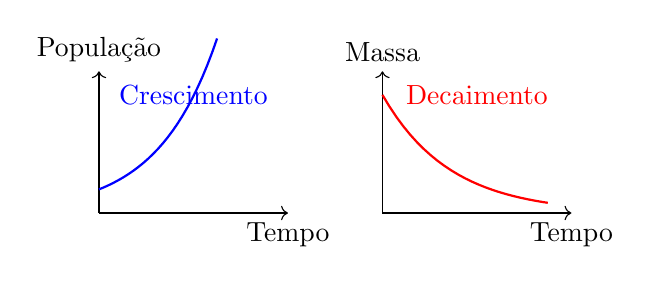
\begin{tikzpicture}[scale=0.6]
    % Crescimento exponencial
    \draw[->] (0,0) -- (4,0) node[below]{Tempo};
    \draw[->] (0,0) -- (0,3) node[above]{População};
    \draw[blue, thick, domain=0:2.5] plot (\x, {0.5*exp(0.8*\x)});
    \node[blue] at (2,2.5) {Crescimento};
    % Decaimento exponencial
    \draw[->] (6,0) -- (10,0) node[below]{Tempo};
    \draw[->] (6,0) -- (6,3) node[above]{Massa};
    \draw[red, thick, domain=0:3.5] plot (\x+6, {2.5*exp(-0.7*\x)});
    \node[red] at (8,2.5) {Decaimento};
\end{tikzpicture}
\end{center}

\section*{7. Exercícios Básicos (1-10)}
\begin{enumerate}
    \item Classifique como crescimento ou decaimento:
    \begin{enumerate}[label=\alph*)]
        \item $f(x) = 3^x$
        \item $g(x) = \left(\frac{1}{4}\right)^x$
    \end{enumerate}
    
    \item Determine o valor inicial e a base:
    \begin{enumerate}[label=\alph*)]
        \item $y = 5 \cdot 2^x$
        \item $f(x) = \frac{1}{3} \cdot (0.8)^x$
    \end{enumerate}
    
    \item Calcule:
    \begin{enumerate}[label=\alph*)]
        \item $2^3 \cdot 2^4$
        \item $\frac{5^6}{5^2}$
    \end{enumerate}
    
    \item Esboce os gráficos de:
    \begin{enumerate}[label=\alph*)]
        \item $f(x) = 2^x$
        \item $g(x) = \left(\frac{1}{2}\right)^x$
    \end{enumerate}
    
    \item Resolva as equações:
    \begin{enumerate}[label=\alph*)]
        \item $2^x = 8$
        \item $3^{x-1} = 27$
    \end{enumerate}
\end{enumerate}

\section*{8. Exercícios Intermediários (11-20)}
\begin{enumerate}\setcounter{enumi}{5}
    \item Determine o domínio e imagem:
    \begin{enumerate}[label=\alph*)]
        \item $f(x) = e^x + 1$
        \item $g(x) = -2 \cdot 3^x$
    \end{enumerate}
    
    \item Aplicações:
    \begin{enumerate}[label=\alph*)]
        \item Uma população cresce segundo $P(t) = 1000 \cdot 1.05^t$. Qual o tamanho após 10 anos?
        \item Uma substância decai segundo $m(t) = 50 \cdot 0.8^t$. Quando restará 10g?
    \end{enumerate}
    
    \item Transforme em base $e$:
    \begin{enumerate}[label=\alph*)]
        \item $4^x$
        \item $10^{2x-1}$
    \end{enumerate}
    
    \item Compare as funções:
    \begin{enumerate}[label=\alph*)]
        \item Qual cresce mais rápido: $2^x$ ou $3^x$?
        \item Qual decai mais rápido: $(0.5)^x$ ou $(0.3)^x$?
    \end{enumerate}
    
    \item Problemas:
    \begin{enumerate}[label=\alph*)]
        \item Se $f(x) = a \cdot b^x$ passa por (0,3) e (2,12), encontre $a$ e $b$
        \item Um investimento rende 7\% ao ano. Escreva a função valor futuro
    \end{enumerate}
\end{enumerate}

\section*{9. Exercícios Avançados (21-30)}
\begin{enumerate}\setcounter{enumi}{10}
    \item Resolva as inequações:
    \begin{enumerate}[label=\alph*)]
        \item $2^{x+1} > 16$
        \item $\left(\frac{1}{3}\right)^x \leq 9$
    \end{enumerate}
    
    \item Funções compostas:
    \begin{enumerate}[label=\alph*)]
        \item Se $f(x) = e^{2x}$, calcule $f(\ln 3)$
        \item Determine $f^{-1}(x)$ para $f(x) = 5 \cdot 3^x$
    \end{enumerate}
    
    \item Modelagem:
    \begin{enumerate}[label=\alph*)]
        \item A meia-vida do Césio-137 é 30 anos. Escreva a função decaimento
        \item Se uma cultura bacteriana dobra a cada 2h, quanto tempo para 10x o inicial?
    \end{enumerate}
    
    \item Desafios:
    \begin{enumerate}[label=\alph*)]
        \item Prove que $e^x \geq x + 1$ para todo $x \in \mathbb{R}$
        \item Resolva $2^x + 2^{-x} = 3$
    \end{enumerate}
    
    \item Problemas complexos:
    \begin{enumerate}[label=\alph*)]
        \item Um carro vale \$20,000 e deprecia 15\% ao ano. Quando valerá \$8,000?
        \item A pressão atmosférica $P(h)$ a $h$ km de altitude é $P(h) = P_0 e^{-kh}$. Se a 5km é 60\% de $P_0$, encontre $k$
    \end{enumerate}
\end{enumerate}

\subsection*{Gabarito Parcial}
\begin{tabular}{|c|l|l|}
\hline
\textbf{Questão} & \textbf{Resposta} & \textbf{Questão} \\
\hline
1a) & Crescimento & 16a) & $a=3$, $b=2$ \\
1b) & Decaimento & 16b) & $V(t) = V_0(1.07)^t$ \\
2a) & $a=5$, $b=2$ & 17a) & $x>2$ \\
2b) & $a=\frac{1}{3}$, $b=0.8$ & 17b) & $x \geq -2$ \\
3a) & $128$ & 18a) & $9$ \\
3b) & $625$ & 18b) & $f^{-1}(x) = \log_3(x/5)$ \\
4a) & Gráfico crescente & 19a) & $m(t) = m_0(0.5)^{t/30}$ \\
5a) & $x=3$ & 20a) & $\approx 7.4$ anos \\
5b) & $x=4$ & 20b) & $k \approx 0.102$ \\
\hline
\end{tabular}

\end{multicols}

\end{document}
